% specifies the documnt class. We usually use article but there are others. 
\documentclass[a4paper,12pt,oneside]{book}              

% these are standard packages used for the math symbols
\usepackage{amsmath,amssymb,amsthm, enumitem, hyperref, tabto} 
\usepackage[T1]{fontenc}
\usepackage[utf8]{inputenc}
\usepackage[english]{babel}
\usepackage{fancyhdr}
\usepackage{lastpage}
\usepackage[pdftex]{graphicx}
\usepackage{float}
\graphicspath{ {./Photos/} }

% These commands below is to make sure the numbering of these are consistent with theorem
% If you are not sure what something means, delete them, build a new file and see the
% difference between the files. You can ignore this part for now.
\newtheorem{theorem}{Theorem}[section]
\newtheorem{conjecture}[theorem]{Conjecture}
\newtheorem{observation}[theorem]{Observation}
\newtheorem{definition}[theorem]{Definition}
\newtheorem{corollary}[theorem]{Corollary}
\newtheorem{lemma}[theorem]{Lemma}
\newtheorem{example}[theorem]{Example}
\newtheorem{remark}[theorem]{Remark}
\newtheorem{notation}[theorem]{Notation}

% Title of your project
\title{%
  \Huge Ramanujan's Square \\
  \LARGE Detailed Analysis\\
  \Large A DV2136 Project \\
  \large Term Report}

% The author command places text right after title
\author{by \\
\Large Afzal (h1810003) \\
\Large Prannaya Gupta (h1810124) \\
\Large Yap Yuan Xi (h1810166) \\
}

\date{\Large July - September 2019}

\begin{document}
\maketitle

\tableofcontents

\part{An Introduction}

\chapter{Contextualisation}
\section{Why are we doing this?}
We are doing this for our DV2136 Junior Math Project, where we are trying to use this concept to test our skill in the Mathematics. We are also doing this because we are interested in Maths and want to see if we can make something out of what we are given.

\section{Inspiration}
We are working on The Magic Squares because it is a fascinating phenomenon. Being such a fluid structure, that is variable based on just a certain number of dates inputted. Its an interesting concept and we really want to build upon it. We want to extend on this concept so we can see what may behold. We want to try. And we want to see if this paper bears any fruit at all.

\newpage
\section{Magic Squares - A Full-Text Description}

\subsection{Abstract}
In real life situations, some problems relating to division of objects equal in numbers and value can be easily solved by constructing a semi magic square or a magic square in accordance with the given conditions. Mathematics is magic if we can either use one formula for a wide range of applications or the formula itself will produce magic properties.

\subsection{A Brief History of the Magic Square}
Magic squares were known to Chinese mathematicians, and Arab mathematicians, possibly as early as the $7^{th}$ century, when the Arabs conquered northwestern parts of the Indian subcontinent and to learned Indian mathematicians and astronomers, including other aspects of combinatorical mathematics. ‘Cornelius Agrippa’ (1486 B.C. to 1535 B.C.) of China is believed to be the first for construction of magic squares.

\subsection{The Properties of a general Magic Square}
A general Magic Square is the arrangement of random number within the cell such that sum of each row = each column = each diagonal. The common sum is known as ‘Magic Constant’ or ‘Magic Number’. If the above condition is valid only for the sum of elements of rows and columns and not for the diagonal elements, then that array is known as a semi magic square. All magic squares are semi magic squares. A normal magic square contains the integers from 1 to $n^2$. The constant sum in every row, column and diagonal is called the magic constant or magic sum, S. The magic constant of a normal magic square with continuous numbers depends only on n and has the value $S = \frac{n(n^2+1)}{2}$.

\subsection{The Area of Our Investigation}
We are trying to investigate The Ramanujan's Magic Square, a magic square devised by the genius mathematician Srinivasa Ramanujan which has a number of exciting properties.

\newpage
\section{Ramanujan: The Man Who Knew Infinity}
\tab Born in 1887, Ramanujan was a young Indian student.
By the age of 23 Ramanujan was making important new discoveries in mathematics. Professor G.H. Hardy recognised a touch of pure genius in Ramanujan’s theorems. Hardy recognised his talents and arranged to bring Ramanujan to England. Ramanujan decided to accept Hardy’s offer, and on 17 March, 1914 he set out by ship to England.
\subsection{England}
In Cambridge, the young Indian set about working on hundreds of new theorems. Hardy said: “I have never met Ramanujan’s equal.”\cite{studyMagicSquare} However, Ramanujan did not fare so well in his private life. His fragile health suffered. He even became suicidal.
Sadly, Ramanujan never regained his health. He died on 20 April, 1920 in a care home near Madras (now Chennai). He continued working on new theorems even on his death bed. Showing his true Mathematical spirit.\cite{historyRamanujan}

\part{The Beginning : An analysis of our options}

\chapter{How does Ramanujan's Magic Square work?}

\section{What are we looking at? - Primary Basis of our Investigation}
\tab We are investigating Srinivasa Ramanujan's Magic Square. It is noticed that in a normal magic square the columns and rows give the same sum. However in this Magic Square, there are other ways to get the same sum. Like the corners, the diagonals and many more.

\subsection{What we can derive from the square}
\tab This is very intriguing to us and made us want to find out how it works and how this is possible. We want to explore the magic of this mathematical square.

\newpage
\section{Description}
\tab This square has a huge number of possible magic square possibilities. You can consider a huge amount magic square patterns like 'By Row', 'By Column', 'By Quarter'.  Below is a definitive list:

\begin{itemize}
  \item The sum of any column is a number y
  \item The sum of any row is the number y
  \item The sum of any diagonal is the number y
  \item The sum of any 2x2 is the number y (except for those in the middle two columns)
\end{itemize}

However, the real miracle of this square its ability to seemingly morph from one's birthday. The main magic square used as an example is actually derived from Ramanujan's birth date, 22 December 1887, thus amounting the sum y as 139. This is an interesting graphic and provides a majorly interesting phenomenon.

\section{Graphical Representation}
\begin{figure}[H]
\begin{center}
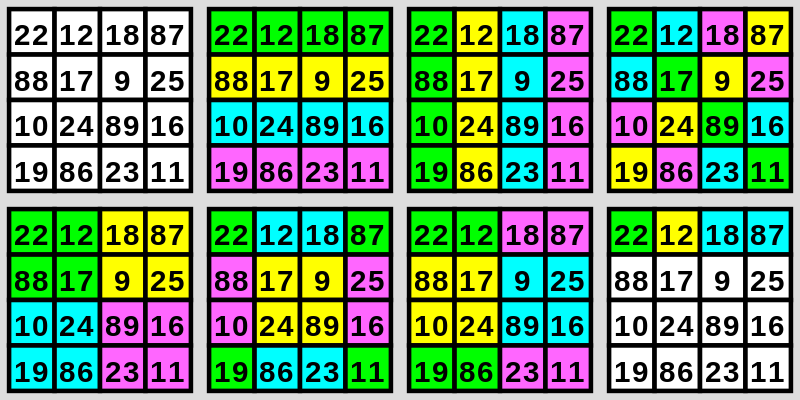
\includegraphics[scale = 0.4]{MagicSquare} 
\cite{magicSquare}
\caption{These diagrams show the ways in which the numbers of the Square add up to 139 in the main Ramanujan Square}
\end{center}
\end{figure}

\newpage
\section{Explanation}
\begin{figure}[H]
\begin{center}
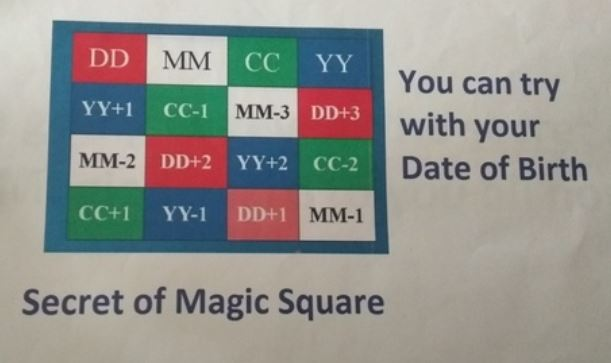
\includegraphics[scale = 1.0]{RamanujanSquare}
\cite{ramanujanSquare}
\caption{This diagram shows the algorithm by which the numbers of the Square add up to 139 in the main Ramanujan Square}
\end{center}
\end{figure}

\paragraph{
Let Me Explain: Consider the first row being the derivation.
}
\begin{equation*}
Sum_{given} = DD + MM + CC + YY
\end{equation*}
where DD is the date, MM is the month, CC is the century and YY is the year.

\paragraph{Now consider the first column.}
\begin{equation*}
Sum_{col_1} = DD + (MM-2) + (CC+1) + (YY+1) = DD + MM + CC + YY
\end{equation*}
\subparagraph{Therefore, $Sum_{col_1} = Sum_{given}$}

\paragraph{If you see, this applies for every single property we showed, because the numbers are perfectly balanced.}
\chapter{What will we try to investigate?}

\section{The Theory of Everything (for RMS)}
Is there really a way to sieve out a Ramanujan's Square using algorithmic problem solving separate from the original?

\section{Broken Time: Dimension of Hour}
Is there another dimension to this magic square? If so, what is it?
    \subsection{5x5 Magic Squares}
        Letting H, D, M, C, Y be the hour, the day, the month, the century and the year respectively. \\
        \def\arraystretch{2}
        \begin{center}
            \begin{tabular}{c|c|c|c|c}
                \hline
                 H + 0 & D + 0 & M + 0 & C + 0 & Y + 0  \\
                 \hline
                 D - 2 & C + 1 & Y + 1 & M + 3 & M - 3 \\
                 \hline
                 Y + 2 & M - 1 & D - 1 & H - 2 & C + 2 \\
                 \hline
                 M - 3 & H + 1 & C - 3 & Y + 2 & D + 3 \\
                 \hline
                 C + 3 & Y - 1 & H + 3 & D - 3 & M - 2 \\
                 \hline
            \end{tabular}
        \end{center}
    \subsection{6x6 Magic Squares}
        Letting m, H, D, M, C and Y be the minute, the hour, the day, the month, the century and the year respectively. \\
        \def\arraystretch{2}
        \begin{center}
            \begin{tabular}{|c|c|c|c|c|c|}
                \hline
                 m + 0 & H + 0 & D + 0 & M + 0 & C + 0 & Y + 0  \\
                 \hline
                 M - 1 & Y + 1 & H - 3 & C + 3 & m - 2 & D + 2\\
                 \hline
                 D + 3 & m - 1 & C - 1 & H + 2 & Y - 2 & M - 1\\
                 \hline
                 Y + 2 & C - 4 & M - 3 & D + 1 & H + 3 & M + 1\\
                 \hline
                 H - 2 & D + 2 & m + 4 & Y - 2 & M - 1 & C - 1 \\
                 \hline
                  \\
                 \hline
            \end{tabular}
        \end{center}

\section{Other Forms: Ultimate Disguise}
Are there any other squares with the same properties?

    \subsection{Variation 1: Diagonal}
        Letting D,M,C,Y be the day, month, century and year of the birthday respectively. \\
        Let start with the diagonal. \\
        \def\arraystretch{2}
        \begin{center}
            \begin{tabular}{|c|c|c|c|}
                \hline
                D + 0 & Y + 2 & M - 1 & C - 1 \\
                \hline
                C - 2 & M + 0 & Y - 1 & D + 3 \\
                \hline
                Y + 1 & D + 1 & C + 0 & M - 2 \\
                \hline
                M + 1 & C - 3 & D + 2 & Y + 0 \\
                \hline
            \end{tabular}
        \end{center}
    \subsection{Variation 2: Box}
        Letting D,M,C,Y be the day, month, century and year of the birthday respectively. \\
        Let start with the Upper Left 2 by 2 square. \\
        \def\arraystretch{2}
        \begin{center}
            \begin{tabular}{|c|c|c|c|}
                \hline
                D + 0 & M + 0 & Y - 1 & C + 1 \\
                \hline
                C + 0 & Y + 0 & M - 3 & D + 3 \\
                \hline
                M - 1 & D + 1 & C + 2 & Y - 2 \\
                \hline
                Y + 1 & C - 1 & D + 2 & M - 2 \\
                \hline
            \end{tabular}
        \end{center}
        
        
    \subsection{Variation 3: Column}
        Letting D,M,C,Y be the day, month, century and year of the birthday respectively. \\
        Let start with the Left most Column. \\
        
        \def\arraystretch{2}
        \begin{center}
            \begin{tabular}{|c|c|c|c|}
                \hline
                D + 0 & C + 2 & Y - 1 & M - 1 \\
                \hline
                M + 0 & Y - 2 & C - 1 & D + 3 \\
                \hline
                C + 0 & D + 2 & M + 1 & Y - 3 \\
                \hline
                Y + 0 & M - 2 & D + 1 & C + 1 \\
                \hline
            \end{tabular}
        \end{center}

\section{Super Asymmetry}
Is there any form of derivation of the overall constant without any symmetrical significance?


\section{A Simple Determinant}
How can we use the determinant for this matrix-like square to identify the possible dates when this is happening?


\bibliographystyle{acm}
\bibliography{MainBib.bib}
\end{document}
